%%---------- Inleiding ---------------------------------------------------------
%
%\section{Introductie}%
\label{sec:introductie}
Veel bedrijven hebben wat men noemt 'een vuilnistabel'. Dit is een tabel met ongestructureerde masterdata. Hierin staan allerlei gegevens door elkaar, waardoor het lastig wordt om iets te doen met deze data. In dit onderzoek zal er gekeken worden naar de verschillende mogelijkheden om data-extractie te verbeteren in zo'n tabellen. Data-extractie of gegevensextractie slaat op het ophalen van relevante gegevens uit een tabel of databank \autocite{Encyclo.nl}. Aan de hand van dit onderzoek zullen bedrijven hun vuilnistabellen veel beter kun gebruiken, of zelfs sorteren, zonder alles handmatig uit te voeren.
\\\indent
In dit onderzoek zal enkel master data onderzocht worden. Master data zijn de gegevens van een bedrijf die niet transactioneel zijn. Dit betekent dat de data niet te maken heeft met transacties zoals het plaatsen van orders bijvoorbeeld. Master data zal wel veranderen in de loop der tijd, maar dit gebeurd zeer langzaam. Eén van de voornaamste voorbeelden hiervan zijn productgegevens: de naam, afmetingen, prijs... Deze gegevens gaan enkel aangepast worden in uitzonderlijke gevallen \autocite{Yellowground}.
\\\indent
Er zijn twee mogelijkheden om deze data op te slaan: gestructureerd of ongestructureerd. Gestructureerde data is georganiseerd en gegroepeerd zodat alle verschillende gegevens in een aparte tabel zitten. Als dit niet het geval is en er bestaat slechts één tabel met daarin allerlei gegevens, is er sprake van ongestructureerde data. Een voorbeeld hiervan is een tabel met de naam, prijs, afmetingen, beschrijving van het product allemaal tezamen \autocite{Seagate}.
\\\indent
Het grote probleem met ongestructureerde master data is het feit dat het verbeteren van de datakwaliteit een stuk moeilijker wordt. Zoeken of sorteren in zo'n tabel is heel moeilijk, ook duplicaten onderscheiden is niet gemakkelijk. Daarnaast kan het soms zelfs lastig worden om de gewenste data op te halen uit zo'n tabel.
\\\indent
In dit onderzoek zullen er verschillende mogelijkheden vergeleken worden om gelijkaardige waarden uit een tabel te vinden, beter gekend als fuzzymatching \autocite{Silva2022}. Er bestaan al een heleboel technieken en metrieken hiervoor, maar wat als we de tabel eerst gaan onderverdelen in verschillende groepen (Clustering) waarbij het de bedoeling is dat elke groep iets gelijkaardigs heeft zodat er een label aan iedere groep kan gegeven worden (Tagging). De methode clustering + tagging zal worden onderzocht en vergeleken met bestaande algoritmes die gebruik maken van andere technieken.
\\\indent
De vergelijkende studie zal uitgevoerd worden aan de hand van aan tabel met ongestructureerde masterdata afkomstig uit een bestaand bedrijf. Met behulp van libraries in Python zal er vergeleken worden op basis van de volgende zaken: de accuraatheid, de snelheid, de precisie (hoeveelheid van de gevonden duplicaten die correct zijn), de recall (hoeveelheid van de aanwezige duplicaten is gevonden) \autocite{GoogleDevelopers2022}.
%
%---------- Stand van zaken ---------------------------------------------------

\section{State-of-the-art}%
\label{sec:state-of-the-art}

%Twee identieke waarden in een tabel onderscheiden is natuurlijk niet zo moeilijk \autocite{Lievens2022}. Het wordt een stuk lastiger om waarden te identificeren die gelijkend zijn, een groot voorbeeld hiervan zijn typefouten. Het is wel belangrijk om een goed algoritme te kiezen, om zo weinig mogelijk, of in het beste geval geen, vals positieve uitkomsten te krijgen \autocite{Silva2022}.
%\subsection{Levenshtein distance}
%Een eerste mogelijkheid is om gebruik te maken van de 'Levenshtein distance'. Deze metriek bepaalt de afstand tussen twee strings aan de hand van het aantal uit te voeren operaties. Deze operaties zijn: een letter toevoegen of verwijderen en een letter veranderen. Hoe meer operaties er moeten uitgevoerd worden, hoe groter de afstand tussen twee strings \autocite{Wikiversity2022}.
%%\subsection{Hamming distance}
%%Een tweede metriek om de afstand te bepalen is de 'Hamming distance'. Deze metriek transformeert alle karakters in beide strings in hun binaire vorm. Bijvoorbeeld: 'a' wordt '1100001' en 'A' wordt '1000001' \autocite{Includehelp}. De afstand tussen beide strings wordt bepaald aan de hand van het aantal verschillen in de binaire codes van de karakters. De afstand tussen 'a' en 'A' is dus 1, aangezien er slechts één binair karakter verschilt \autocite{Silva2022}.
%\subsection{Damerau-Levenshtein distance}
%Een derde metriek hiervoor heet de 'Damerau-Levenshtein distance'. Deze metriek is quasi hetzelfde als de 'Levenshtein distance', maar met de toevoeging van de transposition-operatie \autocite{Wikiversity2022}. Dit houdt in dat twee karakters die naast elkaar staan, gewisseld kunnen worden en de afstand slechts met één verhoogt . Zo wordt de afstand met deze metriek tussen 'over' en 'voer' één, terwijl de 'Levenshtein distance' tussen deze woorden twee zou zijn \autocite{Pypi2020}.
%\subsection{Affine gap distance}
%Een vierde metriek is de 'Affine gap distance'. Hierbij wordt er rekening gehouden met afkortingen, dit komt voornamelijk voor bij namen: 'K. Dehandschutter' in plaats van 'Kobe Dehandschutter'. Met vorige metrieken zou de afstand hiertussen zeer groot zijn, aangezien er drie letters toegevoegd moeten worden, terwijl de twee strings eigenlijk heel gelijkaardig zijn \autocite{Walgran2019}. Qua scoring werkt het als volgt: voor elk eerste karakter dat moet aangepast worden, de opening van de gap, wordt er plus één gedaan en voor elke opvolger in de gap plus een halfje \autocite{Lievens2022}.
%\\\indent
%Bovenstaande afstandsmetrieken zijn allemaal character-based, deze zijn handig om typefouten te ontdekken, maar als er bijvoorbeeld 'Kobe Dehandschutter' en 'Dehandschutter Kobe' wordt vergeleken, gaat de afstand heel groot zijn. Hiervoor is er een nieuwe categorie: de Token-based techniek.
%\subsection{atomic strings}
%Binnen deze techniek zijn er twee metrieken die zullen worden onderzocht. Als eerste is er een algoritme op basis van atomic strings, dit zijn delen van een langere string die gesplitst worden door punctuatie. Er wordt gezegd dat twee atomic strings een overeenkomst opleveren wanneer ze gelijk zijn, of de ene is een prefix van de andere. Zo is 'Deh' een prefix van 'Dehandschutter'. Om de afstand tussen twee strings te berekenen worden beide opgesplitst in atomic strings. Vervolgens wordt het aantal overeenkomsten gedeeld door het gemiddeld aantal atomic strings \autocite{Lievens2022}.
%\subsection{word2vec}
%Waar met voorgaande algoritmes nog geen rekening mee werd gehouden, is de semantiek van de woorden. 'Frigo' en 'Koelkast' bijvoorbeeld, gelijken qua karakters totaal niet op elkaar, maar betekenen eigenlijk wel hetzelfde. Om de similariteit van deze strings te berekenen, wordt elk woord omgezet in een vector via het algoritme word2vec. Vervolgens wordt de cosinusgelijkheid van de vectoren berekend om de afstand tussen de twee woorden te bepalen \autocite{Lievens2022}.
%\subsection{Clustering}
%\subsubsection{K-means}
%Het K-means clustering algoritme wordt gebruikt om te clusteren in een tabel met ongestructureerde data. Er moet op voorhand opgegeven worden hoeveel clusters er nodig zijn, dit is het natuurlijke getal K. Vervolgens worden er K zwaartepunten (centers) geïnitialiseerd op een random positie. Daarna wordt er voor alle waarden berekend bij welk zwaartepunt ze het dichtste liggen en aan die cluster toegevoegd. Vervolgens start een iteratief proces waarbij voor iedere cluster het zwaartepunt wordt verlegt naar het middelpunt. Nu wordt opnieuw voor iedere waarde in de tabel berekend bij welk zwaartepunt ze het dichtst ligt en zo worden opnieuw clusters gevormd. Dit iteratief proces blijft doorgaan totdat de zwaartepunten niet meer verplaatsen en de uiteindelijke clusters gevormd zijn. De dataset zal in K clusters verdeeld zijn. Een groot nadeel van dit algoritme is dat het getal K op voorhand moet vastliggen, terwijl het juist zeer belangrijk is dat dit getal goed gekozen wordt. Hiervoor is er ook een oplossing, namelijk gebruik maken van canopy clustering. Dit is ook een clustering algoritme dat zeer snel uitgevoerd wordt, maar niet zo accuraat is. Wat wel positief is aan dit algoritme, is dat hier K niet op voorhand moet bepaald worden. Hierdoor kunnen we eerst de canopy clustering uitvoeren en aan de hand van de K die hier gebruikt wordt, het K-means algoritme uitvoeren \autocite{Vandenbussche2016}.
%
%
%

Dit onderzoek zal uitgevoerd worden aan de hand van machine learning. Er bestaan drie verschillende types machinelearning-algoritmen. Als eerste is er het gesuperviseerd leren: hierbij zal er aan iedere waarde, de identiteit al worden meegegeven. Simpel voorbeeld: als er een algoritme gesuperviseerd wordt getraind  om katten te herkennen op foto's, dan zal iedere foto die wordt getoond aan het algoritme een label bevatten met 'ja' of 'nee'. Als het algoritme dan goed genoeg getraind is, zal het in staat zijn om foto's zonder label, het juiste label te geven.
Het tweede type is ongesuperviseerd leren. Dit is logischerwijs het omgekeerde van gesuperviseerd leren. In ons simpel voorbeeld van de katten, zal het algoritme een grote dataset met foto's ontvangen. Deze zal dan in die set naar iets zoeken dat overeenkomt in veel van de foto's. Deze overeenkomst wordt in de ogen van het algoritme de 'kat'. Vervolgens splitst het de foto's in twee groepen. Eén die de 'kat' wel bevat en één die hem niet bevat. Aangezien er geen labels hangen aan de dataset, kan het algoritme zelf niet weten of het juist of fout is. Dit zorgt ervoor dat er minder controle is over de uitkomst, waardoor deze methode minder succesvol is. Zo kan het natuurlijk gebeuren dat veel foto's, naast een kat, ook een boom bevatten. Hierdoor kan het gebeuren dat het algoritme de foto's splitst in een groep met boom en zonder boom, want het algoritme kan niet weten hoe een kat eruitziet, hierdoor denkt het misschien dat een boom eigenlijk een kat is. Waarom zou ongesuperviseerd leren dan gebruikt worden als het minder succesvol is? In het voorbeeld van de katten is inderdaad niet zo moeilijk om een label 'ja' of 'nee' aan iedere foto te geven, maar in heel veel andere gevallen kunnen er geen labels aan de data gegeven worden en zou het enorm handig zijn als het algoritme gewoon de data zonder labels in verschillende groepen zou verdelen. Dit geeft al veel inzicht in de data.
Het derde type is reinforcement leren. Dit wordt veel gebruikt bij situaties waarin het algoritme een juiste volgorde van acties moet uitvoeren. Iedere keer dat het algoritme correct is, wordt het beloont. Deze methode wordt ook gebruikt voor het aanleren van gedrag bij dieren. Als een hond getraind wordt om te zitten bijvoorbeeld, krijgt hij een snoepje of aaitje iedere keer hij het commando goed uitvoert.
%{https://ericpostma.nl/publications/AI_Postma2019NL.pdf}

In dit onderzoek wordt gebruik gemaakt van een ongestructureerde masterdata. Dit betekent dat de data geen labels bevat. De bedoeling is om de data te onderverdelen in gelijkaardige groepen. Het is dus vanzelfsprekend dat dit onderzoek zal gebeuren aan de hand van ongesuperviseerd leren.

Nu er beslist is dat er gebruik gemaakt zal worden van ongesuperviseerd leren, komt een volgend probleem naar boven. Onze ongestructureerde masterdata bevat woorden en karakters, maar de algoritmen kunnen dit niet groeperen. Deze verwachten de data in getallen. Een eerste stap in dit onderzoek, is dus het omzetten van de data in getallen of vectoren, dit zijn enorm grote reeksen getallen. Er zijn verschillende manieren om dit te doen.
\subsection{Levenshtein distance}
Een eerste mogelijkheid is om gebruik te maken van de 'Levenshtein distance'. Deze metriek bepaalt de afstand tussen twee strings aan de hand van het aantal uit te voeren operaties. Deze operaties zijn: een letter toevoegen of verwijderen en een letter veranderen. Hoe meer operaties er moeten uitgevoerd worden, hoe groter de afstand tussen twee strings %\autocite{Wikiversity2022}.

\subsection{word2vec}
Waar met de Levenshtein distance nog geen rekening mee wordt gehouden, is de semantiek van de woorden. 'Frigo' en 'Koelkast' bijvoorbeeld, gelijken qua karakters totaal niet op elkaar, maar betekenen eigenlijk wel hetzelfde. Om de similariteit van deze strings te berekenen, wordt elk woord omgezet in een vector via het algoritme word2vec. Vervolgens wordt de cosinusgelijkheid van de vectoren berekend om de afstand tussen de twee woorden te bepalen %\autocite{Lievens2022}.

\subsection{tf-idf}
%{https://www.capitalone.com/tech/machine-learning/understanding-tf-idf/}
Een derde mogelijkheid is tf-idf, dit staat voor term frequency-inverse document frequency. Eerst en vooral hebben we term frequency. Dit is het aantal keer dat een woord voorkomt in het document. Dit kan berekend worden door gewoonweg te tellen hoeveel keer het voorkomt, maar als de documenten maar een paar worden bevatten, zoals in ongestructureerde masterdata toch vaak het geval is, kan dit ook berekend worden aan de hand van een boolean. Het wordt dus 1 als het document het woord bevat en 0 als het woord er niet in voorkomt. Vervolgens is er de inverse document frequency. Dit is een berekening van hoe zeldzaam het woord is ten opzichte van alle documenten in de dataset. Dit is noodzakelijk, want anders zullen woorden zoals 'het', 'een', 'is' of 'er' altijd naar boven komen als veelgebruikte woorden. De bedoeling is dus om de woorden die niet veel voorkomen in alle documenten, maar wel regelmatig in een bepaald document voorkomen, een hoge score te geven. De idf voor een bepaald woord (t) in een dataset (D) wordt als volgt berekend: de logaritme van N, waarbij N gelijk is aan het aantal documenten (d), gedeeld door het aantal documenten waarin het woord (t) voorkomt.
% TODO: \usepackage{graphicx} required


\begin{figure}[h]
    \centering
    \caption{}
    \label{fig:idf-formule}
    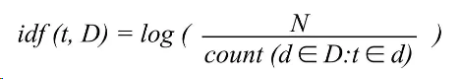
\includegraphics[width=0.7\linewidth]{../foto's/idf-formule}
\end{figure}

Wanneer de tf en de idf berekend zijn, moeten deze nog samengevoegd worden natuurlijk. Dit wordt simpelweg gedaan door de twee waarden te vermenigvuldigen. Hoe hoger de uitkomst is, hoe belangrijker het woord is, als de uitkomst dicht bij 0 ligt is dit woord totaal niet belangrijk.


\subsection{Clustering}
Nu alle data uit de dataset omgezet zijn in vectoren, kan er begonnen worden met clusteren. Hiervoor zullen drie verschillende methoden gebruikt worden. K-means, Hierarchisch en dbscan.

\subsubsection{K-means}
Het K-means clustering algoritme wordt gebruikt om te clusteren in een tabel met ongestructureerde data. Er moet op voorhand opgegeven worden hoeveel clusters er nodig zijn, dit is het natuurlijke getal K. Vervolgens worden er K zwaartepunten (centers) geïnitialiseerd op een random positie. Daarna wordt er voor alle waarden berekend bij welk zwaartepunt ze het dichtste liggen en aan die cluster toegevoegd. Vervolgens start een iteratief proces waarbij voor iedere cluster het zwaartepunt wordt verlegt naar het middelpunt. Nu wordt opnieuw voor iedere waarde in de tabel berekend bij welk zwaartepunt ze het dichtst ligt en zo worden opnieuw clusters gevormd. Dit iteratief proces blijft doorgaan totdat de zwaartepunten niet meer verplaatsen en de uiteindelijke clusters gevormd zijn. De dataset zal in K clusters verdeeld zijn. Een groot nadeel van dit algoritme is dat het getal K op voorhand moet vastliggen, terwijl het juist zeer belangrijk is dat dit getal goed gekozen wordt. Hiervoor is er ook een oplossing, namelijk gebruik maken van canopy clustering. Dit is ook een clustering algoritme dat zeer snel uitgevoerd wordt, maar niet zo accuraat is. Wat wel positief is aan dit algoritme, is dat hier K niet op voorhand moet bepaald worden. Hierdoor kunnen we eerst de canopy clustering uitvoeren en aan de hand van de K die hier gebruikt wordt, het K-means algoritme uitvoeren %\autocite{Vandenbussche2016}.

\subsubsection{dbscan}
Dbscan is de afkorting voor Density-based spatial clustering of applications with noise en dit is een clustering algoritme dat ontstaan is om nested clusters, goed te kunnen berekenen. Dit zijn clusters die gedeeltelijk of zelfs helemaal omringt zijn door een andere cluster. Dit is het algoritme dat het dichtst in de buurt komt met hoe het menselijk oog clustert. Dbscan gaat als volgt te werk: eerst telt het voor iedere waarde, het aantal punten die dicht in de buurt liggen. Dit wordt simpelweg gedaan door een cirkel te trekken rond het punt en vervolgens alle punten die volledig of gedeeltelijk in de cirkel liggen te tellen. De straal van de cirkel is één van de twee parameters die op voorhand zal moeten meegegeven worden. De tweede parameter is het aantal dichte buren een punt nodig heeft om een Core Point te worden. Stel dat dit aantal vier is, dan worden alle punten die vier of meer punten in hun cirkel hebben een Core Point. Dit zijn meestal de punten die in het midden van een cluster liggen. Vervolgens start het algoritme bij een willekeurig Core Point en dit wordt aan de eerste cluster toegevoegd. Daarna worden zijn buren bekeken en alle Core Points daarvan worden ook aan de cluster toegevoegd. Voor ieder toegevoegd punt, wordt deze stap uitgevoerd, tot er geen meer bij kunnen. Vervolgens worden voor ieder punt uit de cluster, zijn buren die geen Core Points zijn ook toegevoegd, maar hun buren, die niet meer. Dit is de eerste cluster, nu wordt er terug gestart bij een willekeurig Core Point die nog niet tot een cluster behoort. Op het einde, als er geen Core Points meer overblijven, kan het zijn dat er nog punten zijn die niet tot een cluster behoren. Deze zijn de uitschieters.

%{https://www.youtube.com/watch?v=RDZUdRSDOok}


%%Hier beschrijf je de \emph{state-of-the-art} rondom je gekozen onderzoeksdomein, d.w.z.\ een inleidende, doorlopende tekst over het onderzoeksdomein van je bachelorproef. Je steunt daarbij heel sterk op de professionele \emph{vakliteratuur}, en niet zozeer op populariserende teksten voor een breed publiek. Wat is de huidige stand van zaken in dit domein, en wat zijn nog eventuele open vragen (die misschien de aanleiding waren tot je onderzoeksvraag!)?
%
%Je mag de titel van deze sectie ook aanpassen (literatuurstudie, stand van zaken, enz.). Zijn er al gelijkaardige onderzoeken gevoerd? Wat concluderen ze? Wat is het verschil met jouw onderzoek?

%Verwijs bij elke introductie van een term of bewering over het domein naar de vakliteratuur, bijvoorbeeld~\autocite{Hykes2013}! Denk zeker goed na welke werken je refereert en waarom.

%Draag zorg voor correcte literatuurverwijzingen! Een bronvermelding hoort thuis \emph{binnen} de zin waar je je op die bron baseert, dus niet er buiten! Maak meteen een verwijzing als je gebruik maakt van een bron. Doe dit dus \emph{niet} aan het einde van een lange paragraaf. Baseer nooit teveel aansluitende tekst op eenzelfde bron.
%
%Als je informatie over bronnen verzamelt in JabRef, zorg er dan voor dat alle nodige info aanwezig is om de bron terug te vinden (zoals uitvoerig besproken in de lessen Research Methods).

% Voor literatuurverwijzingen zijn er twee belangrijke commando's:
% \autocite{KEY} => (Auteur, jaartal) Gebruik dit als de naam van de auteur
%   geen onderdeel is van de zin.
% \textcite{KEY} => Auteur (jaartal)  Gebruik dit als de auteursnaam wel een
%   functie heeft in de zin (bv. ``Uit onderzoek door Doll & Hill (1954) bleek
%   ...'')

%Je mag deze sectie nog verder onderverdelen in subsecties als dit de structuur van de tekst kan verduidelijken.

%---------- Methodologie ------------------------------------------------------
%\section{Methodologie}%
%\label{sec:methodologie}
%
%Het onderzoek zal uit vier verschillende fasen bestaan.
%\\\indent
%Vooraleer er kan begonnen worden met algoritmes uitvoeren, moeten de requirements opgesteld worden waaraan voldaan moet worden, dit wordt dus de eerste fase. Er zal gewerkt worden met de MoSCoW methode (Must have, Should have, Could have, Won't have). Op deze manier is het duidelijk wanneer een algoritme geschikt is en wanneer niet.
%\\\indent
%In de tweede fase zullen alle algoritmes in de long list van gevonden mogelijkheden voor fuzzymatching uitgeprobeerd worden op de gekregen dataset. Zo zal er al een eerste onderscheiding gemaakt kunnen worden tussen degene die geschikt zijn en degene die niet geschikt zijn. Deze opsplitsing gebeurt aan de hand van de opgestelde requirements. Vervolgens wordt kort gekeken waarom de gefaalde algoritmes niet geschikt zijn voor deze probleemstelling, was dit verwacht of totaal niet?
%\\\indent
%Hierna komt de derde fase en nu zullen de algoritmes uit de short list van geschikt algoritmes vergeleken worden. Eerst en vooral wordt er gekeken naar de accuraatheid. Dit wordt berekend door het aantal correcte uitkomsten te delen door het totaal aantal uitkomsten. Dit is één van de belangrijkste eigenschappen van een algoritme, aangezien de resultaten toch correct moeten zijn. Vervolgens worden de precisie en recall vergeleken aangezien deze op een gelijkaardige manier te berekenen zijn. Het is natuurlijk ook belangrijk dat het uitvoeren van een algoritme niet te lang duurt, een volgende eigenschap die zal worden vergeleken is de snelheid van het algoritme.
%\\\indent
%In de vierde en laatste fase zal er een proof-of-concept worden opgesteld voor deze probleemstelling. Het algoritme dat in de vorige fase als meest geschikt naar voor kwam, zal worden gebruikt om aan te tonen of het probleem wel of niet oplosbaar is.
%





%Hier beschrijf je hoe je van plan bent het onderzoek te voeren. Welke onderzoekstechniek ga je toepassen om elk van je onderzoeksvragen te beantwoorden? Gebruik je hiervoor literatuurstudie, interviews met belanghebbenden (bv.~voor requirements-analyse), experimenten, simulaties, vergelijkende studie, risico-analyse, PoC, \ldots?
%
%Valt je onderwerp onder één van de typische soorten bachelorproeven die besproken zijn in de lessen Research Methods (bv.\ vergelijkende studie of risico-analyse)? Zorg er dan ook voor dat we duidelijk de verschillende stappen terug vinden die we verwachten in dit soort onderzoek!
%
%Vermijd onderzoekstechnieken die geen objectieve, meetbare resultaten kunnen opleveren. Enquêtes, bijvoorbeeld, zijn voor een bachelorproef informatica meestal \textbf{niet geschikt}. De antwoorden zijn eerder meningen dan feiten en in de praktijk blijkt het ook bijzonder moeilijk om voldoende respondenten te vinden. Studenten die een enquête willen voeren, hebben meestal ook geen goede definitie van de populatie, waardoor ook niet kan aangetoond worden dat eventuele resultaten representatief zijn.
%
%Uit dit onderdeel moet duidelijk naar voor komen dat je bachelorproef ook technisch voldoen\-de diepgang zal bevatten. Het zou niet kloppen als een bachelorproef informatica ook door bv.\ een student marketing zou kunnen uitgevoerd worden.
%
%Je beschrijft ook al welke tools (hardware, software, diensten, \ldots) je denkt hiervoor te gebruiken of te ontwikkelen.
%
%Probeer ook een tijdschatting te maken. Hoe lang zal je met elke fase van je onderzoek bezig zijn en wat zijn de concrete \emph{deliverables} in elke fase?

%---------- Verwachte resultaten ----------------------------------------------
%\section{Verwacht resultaat, conclusie}%
%\label{sec:verwachte_resultaten}
%
%Er wordt verwacht dat het beste algoritme voor deze probleemstelling K-means wordt. Dit zal de tabel eerst clusteren waarna er via tagging gezocht kan worden naar duplicaten. Door het feit dat de tabel geclusterd wordt, wordt verwacht dat het algoritme sneller gerund kan worden dan anderen en dat het ook correcter kan uitgevoerd worden.



%Hier beschrijf je welke resultaten je verwacht. Als je metingen en simulaties uitvoert, kan je hier al mock-ups maken van de grafieken samen met de verwachte conclusies. Benoem zeker al je assen en de onderdelen van de grafiek die je gaat gebruiken. Dit zorgt ervoor dat je concreet weet welk soort data je moet verzamelen en hoe je die moet meten.
%
%Wat heeft de doelgroep van je onderzoek aan het resultaat? Op welke manier zorgt jouw bachelorproef voor een meerwaarde?
%
%Hier beschrijf je wat je verwacht uit je onderzoek, met de motivatie waarom. Het is \textbf{niet} erg indien uit je onderzoek andere resultaten en conclusies vloeien dan dat je hier beschrijft: het is dan juist interessant om te onderzoeken waarom jouw hypothesen niet overeenkomen met de resultaten.














